\subsection{Testkonzept Software}\label{sec:testkonzeptSoftware}

Erklärt, welcher Teil wie getestet wird und führt die Ergebnisse mit Auswertung auf.


\subsubsection*{LC-Filter}
Die Validierung des LC-Filters wurde mittels eines $500Hz$ Sinus Signals erledigt. Dabei wurde sowohl ohne Filter wie auch mit Filter eine KO Bild aufgenommen. \autoref{fig 500Hz ohne Filter} zeigt das Signal ohne Filter. Rot angezeigt ist die FFT des Signals. In \autoref{fig 500Hz mit Filter} ist das Signal und die FFT davon mit dem LC-Filter. 


\begin{figure}
\center
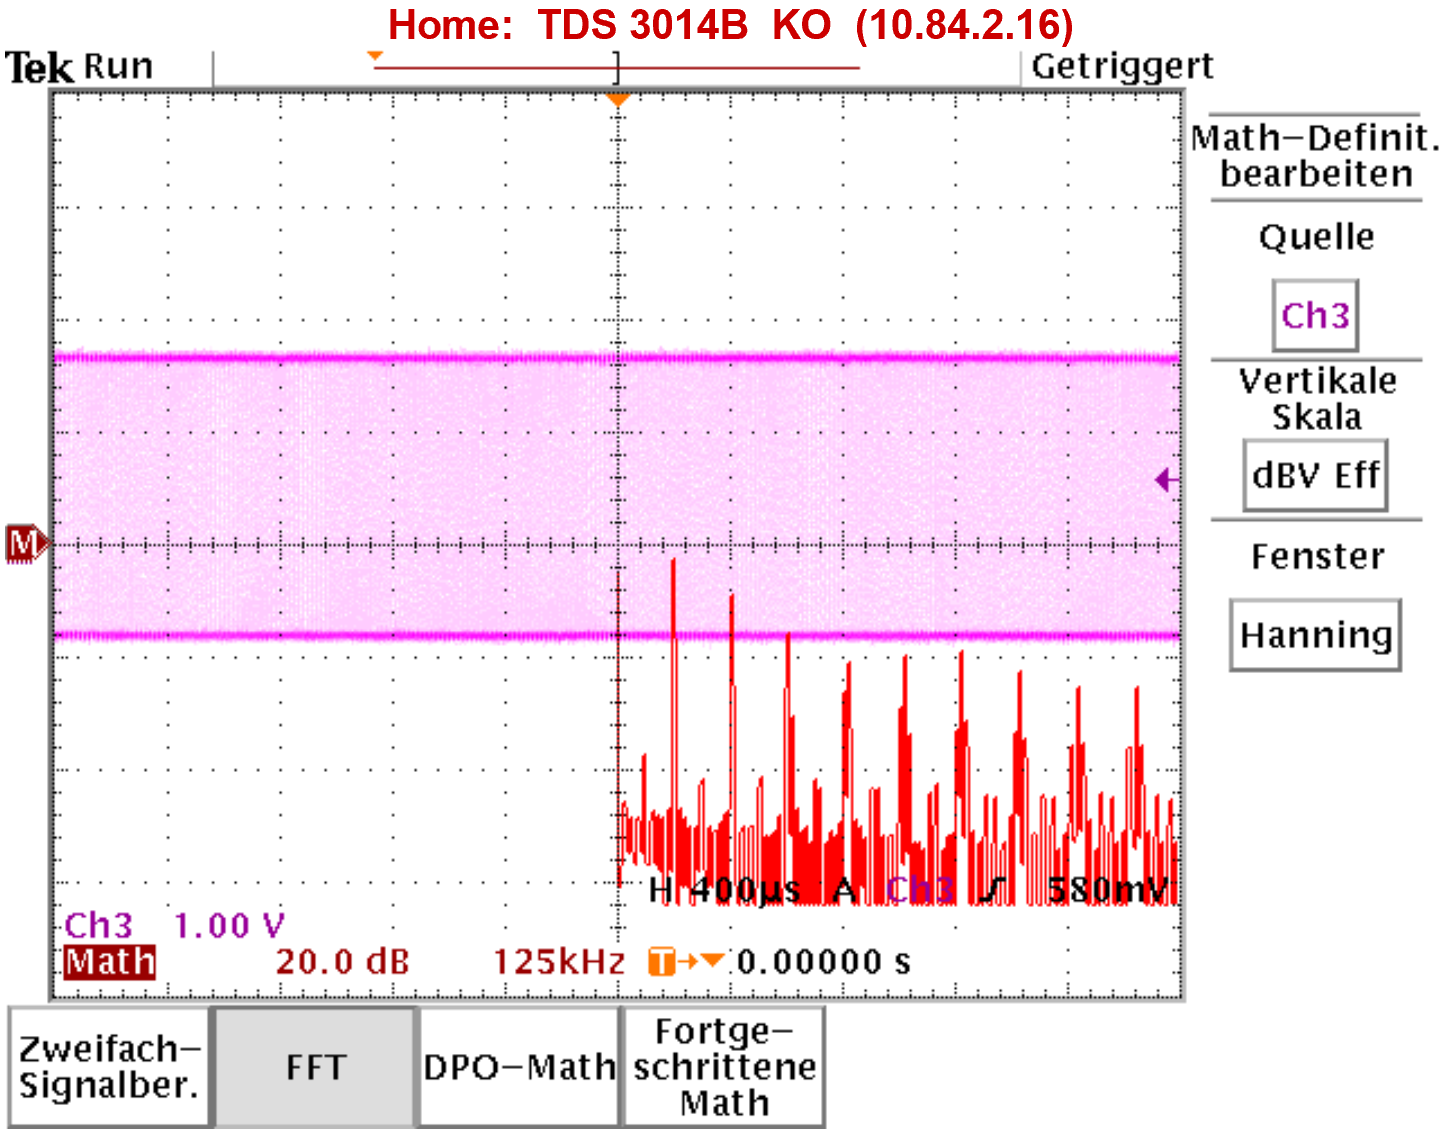
\includegraphics[scale=1.0]{data/500Hz_Sin_ohne_Filter_FFT.png}
\caption{500Hz Sinus Signal und FFT ohne LC-Filter }
\label{fig 500Hz ohne Filter}
\end{figure}

\begin{figure}
\center
\includegraphics[scale=1.0]{data/500Hz_Sin_mit_Filter_FFT.png}
\caption{500Hz Sinus Signal und FFT mit LC-Filter}
\label{fig 500Hz mit Filter}
\end{figure}

Durch die beiden KO Aufnahmen wurde ersichtlich, dass durch den Filter ein deutlich besseres und weniger verrauschtes Signal rekonstruiert wird. Somit ist der LC-Filter notwendig, da mit ihm die Schaltfrequenzen des PWM Ausgangs unterdrückt werden. 